\begin{frame}[t,fragile]{ヒストグラムの作り方}
  \begin{itemize}
    %\setlength{\itemsep}{1em}
  \item 連続変数(実数)のデータの場合 ([]内はサンプルプログラムでの変数名)
    \begin{itemize}
    \item $N$: サンプル数 [{\tt samples}]
    \item $x_{\rm min}$: データの最小値(カットオフ) [{\tt xmin}]
    \item $x_{\rm max}$: データの最大値(カットオフ) [{\tt xmax}]
    \item $n$: ビンの個数 [{\tt bins}]
    \item $\Delta$: ビンの幅 ($\Delta=(x_{\rm max}-x_{\rm min}) / n$) [{\tt dx}]
    \end{itemize}
  \item サイズ$n$の配列を準備
    \begin{itemize}
    \item データ毎にどのビンに入るか計算: $j = (x - x_{\rm min}) / \Delta$
    \item (必要に応じて) $0 \le j < n$であることを確認 (範囲外のデータは無視する)
    \item 配列の$j$番目の値を1増やす
    \end{itemize}
  \item サンプルプログラム: \href{https://github.com/todo-group/computer-experiments/blob/master/exercise/monte_carlo/histogram.c}{histogram.c}

    (コンパイルには\href{https://github.com/todo-group/computer-experiments/blob/master/exercise/include/mersenne_twister.h}{mersenne\_twister.h}と\href{https://github.com/todo-group/computer-experiments/blob/master/exercise/include/cmatrix.h}{cmatrix.h}が必要)
  \end{itemize}
  \vspace*{-5.5cm} \hfill \resizebox{0.28\textwidth}{!}{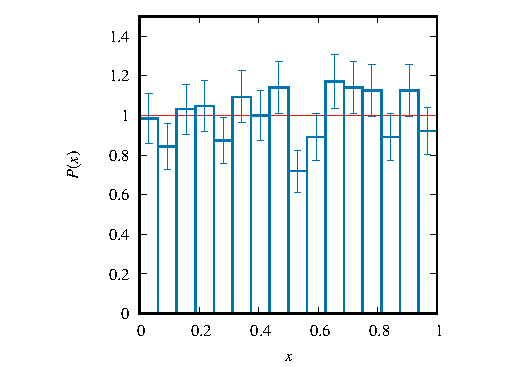
\includegraphics{image/histogram.pdf}}
\end{frame}
